%
% latex-sample.tex
%
% This LaTeX source file provides a template for a typical research paper.
%

%
% Use the standard article template.
%
\documentclass{article}

% The geometry package allows for easy page formatting.
\usepackage{geometry}
\geometry{letterpaper}

% Load up special logo commands.
\usepackage{doc}
\usepackage{cite}

% Package for formatting URLs.
\usepackage{url}

% Packages and definitions for graphics files.
\usepackage{graphicx}
\usepackage{epstopdf}
\DeclareGraphicsRule{.tif}{png}{.png}{`convert #1 `dirname #1`/`basename #1 .tif`.png}

%
% Set the title, author, and date.
%
\title{Usability of Modern Display Technologies}
\author{Rachel Rivera}
\date{October 16, 2014}

%
% The document proper.
%
\begin{document}

% Add the title section.
\maketitle

% Add an abstract.
\abstract{
This study aims to examine how interaction design concepts specifically map to the usability of modern display technology.
//TODO: write a better abstract
}

% Add various lists on new pages.
\pagebreak
\tableofcontents


% Start the paper on a new page.
\pagebreak

%
% Body text.
%
\section{Introduction}
\label{introduction}

The study of electronic screens is significant in the field of human-computer interaction (HCI) as screens are the devices through which information is transferred between the users and the interface. Although electronic displays have been around for nearly a century,\footnote{The cathode ray tube (CRT) was first made commercial in 1922.\cite{Cathode}} they are still transforming and evolving in a multitude of ways. Screens are diversifying in order to tackle the limitations that have presented themselves over the years. 

Screen devices have been changing in size, shape, flexibility, and resolution in order to improve usability for specific tasks. For example, \textit{focus plus context screens}, which are wall-size low-resolution displays with an embedded high-resolution display region, are currently a proposed solution to working with visual documents too large to fit standard screens.\cite{Baudisch} Another kind of screen that is emerging is the \textit{BiDirectional (BiDi) Screen}, which is a thin, depth-sensing liquid-crystal display (LCD) that allows for 3D interaction using light fields.\cite{Hirsch}

 Though each kind of screen has its merits, this study will focus exclusively on touch sensitive screens. Many experts within the field of interaction design have discussed how the concepts of interaction design map specifically to the usability of touch sensitive screens. In a study from Link\"{o}ping University, researchers articulated how ``interaction design on touch sensitive screens is literally the most `direct' form of HCI, where information display and control are but one surface."\cite{Albinsson}


\section{Background/ Prior Work/ Literary Review}
There exists a fair amount of previous work pertaining to the advantages as well as the limitations of touch sensitive screens. One limitation that is often discussed in the literature is how typing on flat surfaces with no physical keys to guide the fingers requires heightened visual attention. A study by Hussain Tinwala and Scott MacKenzie suggests that since the visual demand on the user is increased, concentration is diverted from the thoughts being expressed. \cite{Tinwala:2010:ETE:1868914.1868972} There exist several input entry methods, however, that attempt to address this problem. For instance, Tinwala and MacKenzie present a system that includes auditory and tactile feedback to guide eyes-free entry using speech and non-speech sounds. \cite{Tinwala:2010:ETE:1868914.1868972} Another proposed solution comes from Tactus Technology, a company in Fremont, California. Employees of Tactus Technology are creating a keyboard with shape-shifting keys that pop up from the screen's surface when needed and recede again when no longer necessary.\cite{Tactus} Craig Ciesla, the co-founder of the company, said that the keyboard will be offered later this year. 

\begin{figure}[ht]
\centering
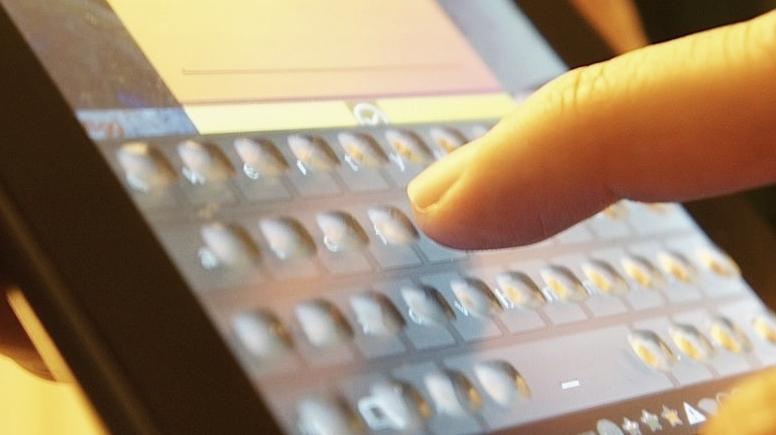
\includegraphics[width=2.7in]{tactus-keyboard.jpg} 
\caption{A Tactus keyboard}
\label{figure-sample}
\end{figure}

Another limitation of touchscreen devices that is frequently examined in the literature is how the human finger as a pointing device has ``very low resolution."\cite{Albinsson} With mobile touch screens in particular, research has illustrated how it is difficult for users to point at targets that are often smaller than the width of their finger. A notable approach to tackling this problem was made by Schneiderman, Sears, and colleagues.\cite{Sears} Their basic technique provides a cursor above the user's finger tip with a fixed offset when touching the screen. The user drags the cursor to a desired target and then lifts the finger to select the targeted object. Although this technique allows users to perform precise movements with generally less errors, the user's efficiency tends to suffer.

Instead of using a bare finger, in some cases the user may use a stylus (pen) to interact with touch screens. A stylus is much ``sharper" pointer than a finger tip, but its resolution may still not be as good as a mouse cursor. A study shows taht pen input is emerging as a promising interaction modality for touch screens.\cite{Bi} The drawbacks to the stylus solution, as discussed in a study by Forlines and Balakrishnan, include the occlusion of other elements on the screen.\cite{Forlines}

Zooming is another method that has been investigated in attempts to increase precision of touchscreen interaction. It is possible to use zooming to enlarge the information space enough so that the user can comfortably point at the target with a bare finger. A common implementation of this zooming technique is called \textit{bounding box zoom}.\cite{Albinsson} With this approach, the user first activates a zooming mode, and then draws a `bounding box' that encloses the area to be zoomed in. When the user releases the box, the system zooms and pans to the selected are and the mode switches back to pointing. One zooming graphical interface that implements the \textit{bounding box zoom} technique is \textit{Pad++}.\cite{Bederson} Though the \textit{Pad++} helps users effectively touch things on the screen, one cost is that ``designers can no longer rely on the users' familiarity with metaphorical reference and this has learnability consequences." \cite{Bederson} 

Some ``Interaction on touch sensitive screens is literally the most `direct' form of HCI, where information display and control are but one surface. The zero displacement between input and output, control and feedback, hand action and eye gaze, make touch screens very intuitive to use, particularly for novice users. Not surprisingly, touch screens have been widely and successfully used in public information kiosks, ticketing machines, bank teller machines, and the like. Besides its directness, touch screen interfaces also have additional advantages. First, because its control surface is overlaid on the display, no extra input control device or space is necessary for touch screen interaction. Second, touch screens are more robust than free moving input devices such as the mouse. Being direct between control and display, touch screens also have special limitations. First, the user's finger, hand, and arm can obscure part of the screen. Second, the human finger as a pointing device has a very low 'resolution'." 

This means less focus on the act of composition. Keys that rise and fall don't use up valuable screen real estate when no longer needed, are a good solution. Accurate typing isn't the only problem with touch screens. Many studies suggest that people's memory and comprehension are often better when they read long passages on paper than on screen, said Mariette DiChristina, editor in chief of Scientific American. But electronic textbooks are incorporating ways to compensate for this.

Perhaps the most important functionality to learn for the paper is \LaTeX\ bibliography support.  Citations and references are handled automatically by \LaTeX\ through its companion program, \BibTeX.  All you have to do is provide a bibliography file that provides the reference information and internal keys (very much like variable names) that you use in your document.\footnote{And always remember to run \LaTeX\ \emph{at least twice} after running \BibTeX.}

Like Section~\ref{introduction}, a background, preliminary, and related work section is also almost certainly needed for your paper.  In this section, describe any history, work, or projects that serve as direct contributors to the subject of your research paper.  Look at other papers in the literature to see how they organized, presented, and discussed prior work.

The Shneiderman/Plaisant text \cite{dui} provide some pointers to seminal or key works; because they made it into the textbook they aren't necessarily ``bleeding edge,'' but they likely provide the foundation for your chosen subject matter.

\section{Main Content Sections}

The outline after the introductory and background, preliminary, and related work sections is more dependent on the specific subject of your research.  Remember to cite references where appropriate, organize the material so that it flows well and is clear to the reader.

\subsection{Multiple Outline Levels}

\LaTeX\ has support for up to three outline levels (\verb!\section!, \verb!\subsection!, and \verb!\subsubsection!).  It also recognizes \verb!\paragraph! and \verb!\subparagraph! directives, though those don't show up in the table of contents.  All of these directives expect a title.

Note also the use of the \verb!\verb! directive for inserting code-like labels or symbols.  It was particularly needed here so that we can include the backslash character in the text.

\subsection{Tables and Figures}

\LaTeX\ has full support for tables and figures.  Table~\ref{table-sample} shows a sample table and Figure~\ref{figure-sample} shows a sample figure.  Note the built-in support for captions and the automated numbering functionality.  Lists of tables and figures can also be automatically generated, as seen at the beginning of this document.

\begin{table}
\centering
\begin{tabular}{|c|c|c|}\hline
Column 1 & Column 2 & Column 3 \\\hline\hline
a & b & c \\
d & e & f \\
g & h & i \\\hline
\end{tabular}

\caption{A sample table}
\label{table-sample}
\end{table}



One very important thing to remember about how \LaTeX\ handles tables and figures by default: you don't have to worry about where they go exactly.  The general rule is that you insert them in the source after your first reference to them, and \LaTeX\ determines their final position.  It also makes decisions on how much page space to devote to them.  This all follows \LaTeX's overall theme of focusing on the content of your paper, and not its format.

Just so you can see a second table, Table~\ref{table-sample2} is provided.

\begin{table}
\centering
\begin{tabular}{|c|c|c|}\hline
Column 1 & Column 2 & Column 3 \\\hline\hline
a & b & c \\
d & e & f \\
g & h & i \\\hline
\end{tabular}

\caption{Another sample table}
\label{table-sample2}
\end{table}

\section{Another Section}

We're adding another section just so you can see how that looks.  Plus there are a few more \LaTeX\ features to illustrate.

\subsection{Bulleted and Numbered Lists}

\LaTeX\ is very good at providing clean lists.  Examples are shown below.

\begin{itemize}
\item Bulleted items come out properly indented and spaced, every time.

\begin{itemize}
\item Sub-bullets are a virtual no-brainer: just nest another \verb!itemize! block.
\item Note how the bullet character automatically changes too.
\end{itemize}

\item Just keep on adding \verb!\item!s\ldots

\item \ldots until you're done.
\end{itemize}

Numbered lists are almost identical, except that you specify \verb!enumerate! instead of \verb!itemize!.  List items are specified in exactly the same way (thus making it easy to change list types).

\begin{enumerate}
\item A list item
\item Another list item
\item A list item with multiple nested lists

\begin{itemize}
\item Nested lists can be of mixed types.
\item That's a lot of power and flexibility for the price of learning a handful of directives.

\begin{enumerate}
\item Like nested bullet lists, nested numbered lists also ``intelligently'' change their numbering schemes.
\item Meanwhile, all \emph{you} have to write is \verb!\item!.  \LaTeX\ does the rest.
\end{enumerate}
\end{itemize}

\item Back to your regularly scheduled list item

\end{enumerate}

\subsection{Subsection with Another Figure}

We may as well include a second figure also, shown in Figure~\ref{figure-sample2}.  The same image file is used, but note how it can be resized.  Again, observe how the positions of the tables and figures do not necessarily match their positions in the source file, reiterating the aforementioned \LaTeX\ functionality for deciding where these items go in the final document.  You provide an approximate location, and \LaTeX\ does the rest.


\section{Conclusion}


Wrap up your paper with an ``executive summary'' of the paper itself, reiterating its subject and its major points.  If you want examples, just look at the conclusions from the literature.
\clearpage


\bibliography{mybib}{}
\bibliographystyle{plain}
\end{document}
%%%%%%%%%%%%% end %%%%%%%%%%%%%%%%%%%%%%%%%%%%%%%


\end{document}
